The next step will be to compare and discuss \codyze{} and \cognicryptsast{} in order to identify how they work in practice. This will include which editors and IDEs they support, what error messages they generate, and how they function in practice. As both tools are capable of analyzing Java programs, we have compared the tools for analyzing Java programs; \codyze's analysis of C++ and C programs is left to future research.

\subsubsection*{Setup}
For this comparison, we used two virtual machines that had the same configuration, which means that they had the same hardware specifications (Intel(R) Xeon(R) CPU E5-2695, 2.30GHz machine with 2 virtual processors, 8 GB RAM, and 50 GB hard disc capacity) and the same operating system (Windows 10 Education). On the first machine we installed Java 8 (JDK version 1.8.0\_301) and on the second Java 11 (JDK version 11.0.11) since \codyze{} requires Java 11 or above while \cognicryptsast{} requires Java 8. The Eclipse 2020-06 was installed on both machines since this is the latest version of Eclipse that supports the two Java versions. 
The versions of \codyze{} and \cognicryptsast{} that we used are not the published versions. We downloaded the source code of \cognicryptsast{} and \codyze{} up to the date of 31st of October 2021 and built them on the first and second virtual machines, respectively. We have downloaded the following source codes.
\cognicrypt{} plugin source code on the develop branch to the commit ef64a0f\footnote{\url{https://github.com/eclipse-cognicrypt/CogniCrypt/commit/ef64a0f2aa7bd54fdc70ae518691cfadf7f47f53}} to use the \cognicryptsast{} as part of \cognicrypt{} Eclipse plugin. In addition, the \cognicryptsast{} standalone command-line tool from the develop branch to this commit 35d0916 \footnote{\url{https://github.com/CROSSINGTUD/CryptoAnalysis/commit/35d09163f97b6919a4359fcaa0e846af95c1fed1}}. Lastly, the source code of \codyze{} main branch to the commit 0468af1\footnote{\url{https://github.com/Fraunhofer-AISEC/codyze/commit/0468af19b90b16353402938db4e326b6dc63c4f7}}.

We will later use the same machines to compare the DSLs in the DSL comparison section (Section \ref{sec:dsl}) and evaluate \codyze{} and \cognicryptsast{} performances in the Evaluation chapter (cf. Chapter \ref{ch:eval}).

\subsection*{Discussion}
Currently, \codyze{} is available in Eclipse, IntelliJ, and Visual Studio with the Language Server Protocol (LSP) technology, while \cognicryptsast{} is only available within Eclipse. \codyze{} will automatically analyze Java, C, and C++ projects upon opening or saving, but there is no button in any of the IDEs for initiating or stopping the analysis. Both tools provide command-line support, \codyze{} also offers an interactive command-line that allows us to explore the CPG on our own.

We were only able to use the \codyze{} plugin in Eclipse and view the results of the analysis. We successfully installed the \codyze{} plugin on IntelliJ and set it up according to the instructions provided on the \codyze{} documentation page \cite{cod}. However, the analysis did not yield any results for any sample code with sufficient correct and incorrect usage of cryptographic APIs. We have also raised an issue on \codyze's Github page concerning this matter\footnote{https://github.com/Fraunhofer-AISEC/codyze/issues/374}.
In the results of \codyze's analysis, in addition to showing violations against the rules, it also alerts when a rule is being used correctly.

We present the results of the \codyze{} and \cognicryptsast{} analyses on the code sample shown in Listing \ref{lst:codesample} in the command-line as a representative example of the analysis results of both tools. \codyze{} command-line tool gets the path to the source code file or a folder of the project, but \cognicryptsast{} command-line tool gets the path to the jar file; therefore, we made a jar file of the sample code.

Figure \ref{fig:codyzecl} shows the result of \codyze's analysis. The result indicates two violations, namely the unspecified provider name and the insecure Cipher algorithm. We will discuss these type of errors in Chapter \ref{ch:eval}. As illustrated in the figure, both errors have the action of INFO, causing \codyze{} to display the violations as information rather than as errors. Likewise, violations are displayed in the IDEs as information rather than errors which may cause confusion because verifications are also displayed as information. This problem has been reported on \codyze's Github page\footnote{https://github.com/Fraunhofer-AISEC/codyze/issues/285}. The name of the violated rule is indicated in the LogMsg. The Location points to the location of the analyzed project.  The exact location in the code where the error occurred is given in the Region. The problem is true if this is an error, and the identifier is the onfail message of the rule that was violated. In the IDEs, the error message will be the error description from findingDescription.json that is described under Section \ref{sec:theotools}. In Figure \ref{fig:codyzecl}, the results are not well-formatted. This is an issue in the version of \codyze{} that we mentioned in the setup of this section. The results were more readable when using \codyze{} version 1.5.5, as shown in Figure \ref{fig:codyzecl15} in the appendices.
\begin{figure}[H]
\centering
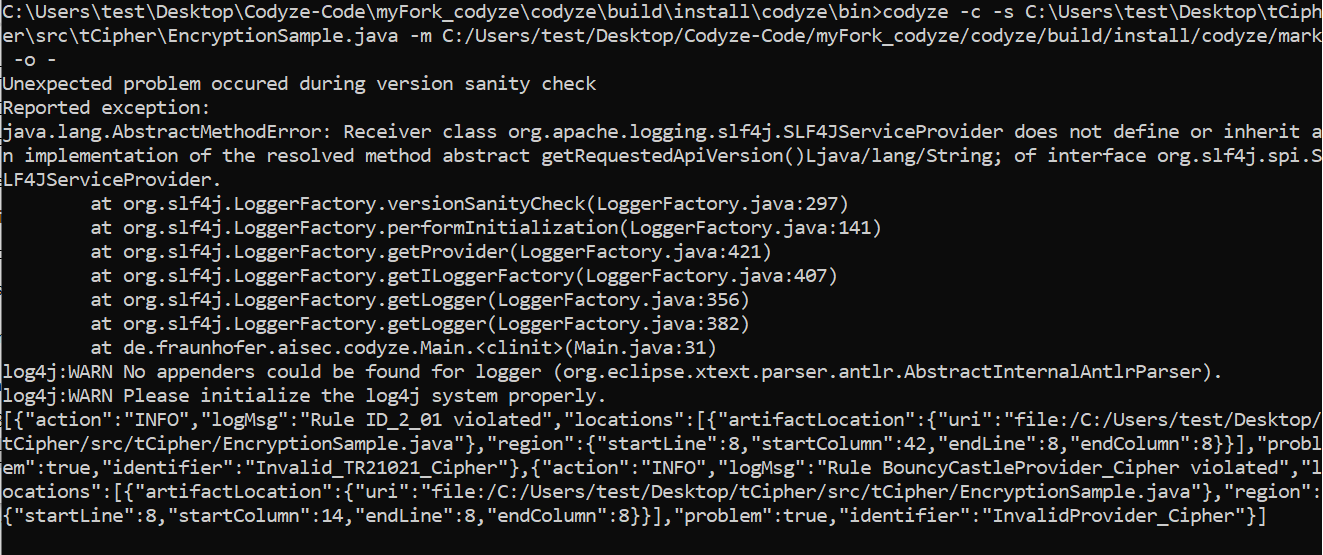
\includegraphics[width=1\linewidth]{thesis/figures/codyzecommand.PNG}
\caption{Result of the analysis of Listing \ref{lst:codesample} by \codyze{} in command-line.}
\label{fig:codyzecl}
\end{figure}

\cognicrypt's plugin provides toolbar and context menu buttons for triggering \cognicryptsast{} and \cognicryptgen{}. Moreover, it provides an option to only analyze the dependencies of a project. Figure \ref{fig:cccl} shows the result of the analysis done by \cognicryptsast{} in command-line. This analysis identified a Constraint error, indicating that the Cipher algorithm was insecure and a RequiredPredicate error, indicating that the key used in the Cipher has not been generated with a proper key generator API. The Figure \ref{fig:cccl} displays the name of the class and the method in which the error occurs. Thereafter, the type of error and the violated rule are displayed. This is followed by the error message and the statement that contains the error. The description of an error generated by \cognicryptsast{} on the command-line and in the Eclipse IDE are similar. 
\begin{figure}[H]
\centering
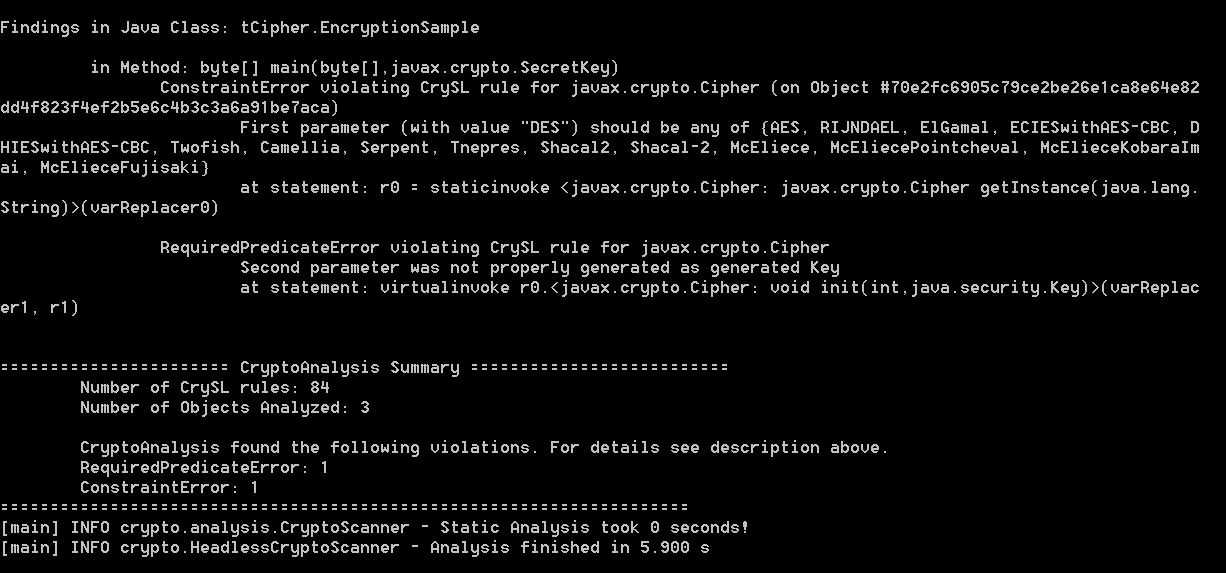
\includegraphics[width=1\linewidth]{thesis/figures/CCCommand.PNG}
\caption{Result of the analysis of Listing \ref{lst:codesample} by \cognicryptsast{} in command-line.}
\label{fig:cccl}
\end{figure}

